%!TEX TS-program = xelatex
%!TEX encoding = UTF-8 Unicode
% !Mode:: "TeX:UTF-8"

\documentclass[a4paper,12pt]{article}
\usepackage[a4paper,hmargin=1in,vmargin=1in]{geometry} % 用Microsoft Office 中Word 的默认页边距
\usepackage{multicol}
\setlength{\columnsep}{1.0cm} %分栏之间的空隙间隔

\usepackage{comment}
\usepackage{ulem} %下划线,强调处理
\usepackage{pifont} %非常有用的特殊符号集合
\usepackage{ xunicode, xltxtra, fancybox, setspace,xcolor}

\usepackage{fontspec}
\newfontfamily\Monaco{Monaco} %自定义指定字体,Monaco字体适用于程序代码

\usepackage[CJKmath=true,CJKchecksingle]{xeCJK}
\XeTeXlinebreaklocale "zh"  
\XeTeXlinebreakskip = 0pt plus 1pt minus 0.1pt  %中文断行
%\xeCJKsetup{AutoFakeBold=true, AutoFakeSlant=true} 
\setCJKmainfont[BoldFont={IPAGothic}]{FZLanTingHeiS-EL-GB} %方正字体,也可以改成:微软雅黑
\setCJKsansfont{FZLanTingHeiS-EL-GB}

%\setCJKmainfont[BoldFont={IPAGothic}]{FZFangSong-Z02}
%\setCJKsansfont{微软雅黑}

\setCJKfamilyfont{Yahei}{微软雅黑}  
\newcommand{\Yahei}{\CJKfamily{Yahei}} 

\newcommand{\Lanting}{\CJKfamily{Lanting}}

\usepackage{amsmath, amsthm, amsfonts, amssymb, mathrsfs} %数学公式相关 amssymb用于斜体字符,如varnothing,  masthm用于定理, mathrsfs用于花体字母

\usepackage{caption, algorithm} %排版伪代码算法使用
\usepackage[]{algpseudocode}

\floatname{algorithm}{\Yahei{算法}}
\renewcommand{\algorithmicrequire}{\Yahei{输入:}} 
\renewcommand{\algorithmicensure}{\Yahei{输出:}}
\renewcommand{\tablename}{表}
\renewcommand{\figurename}{图}
\renewcommand\refname{参考文献}
\renewcommand{\labelenumi}{(\theenumi)}

\usepackage{colortbl, booktabs, multirow, makecell, longtable} %表格处理相关的Package
\usepackage{tabularx}

\usepackage{tikz, flowchart} % tikz绘图
\usepackage{pgfplots}
\usetikzlibrary{decorations.pathreplacing}
\usetikzlibrary{decorations.markings}
\usetikzlibrary{calc, arrows,shapes, shapes.geometric, positioning}
\usetikzlibrary{topaths}
\usetikzlibrary{mindmap}
\usetikzlibrary{matrix}
\newcommand*\circled[1]{\tikz[baseline=(char.base)]{
            \node[shape=circle,draw,inner sep=0.1pt] (char) {#1};}}

\usepackage{indentfirst}  %首行缩进
\setlength{\parindent}{2em} 
\setlength{\listparindent}{2em} %item列表的段落缩进量
\usepackage{enumitem}
\setenumerate[1]{itemsep=0pt,partopsep=0pt,parsep=\parskip,topsep=5pt}
\setitemize[1]{itemsep=0pt,partopsep=0pt,parsep=\parskip,topsep=5pt}
\linespread{1.25} % Change line spacing here, Palatino benefits from a slight
                  % increase by default

\usepackage[numbers]{natbib} %cite style 
\newcommand{\upcite}[1]{\textsuperscript{\textsuperscript{\cite{#1}}}}
\newcommand{\mycite}[1]{\textsuperscript{\textsuperscript{\cite{#1}}}}
%\newcommand{\mycite}[1]{(\citeauthor{#1}, \citeyear{#1})}

\renewcommand\arraystretch{1.2} %表格的高度加大
\setlength{\abovecaptionskip}{-6pt} %缩小表格离标题的空白高度
%\setlength{\belowcaptionskip}{-5pt}
\setlength{\textfloatsep}{1mm}  %缩小表格与后面文字的距离

\captionsetup{belowskip=-10pt}%缩小标题后面的空白
%\captionsetup{aboveskip=0pt}

\renewcommand{\rm}[1]{{\color{blue} \Yahei #1}} %表格的高度加大

\renewcommand{\thefootnote}{\noindent *}
\pagestyle{empty} %去掉页码


\usepackage{titlesec}
\titleformat{\section}
            {\normalfont\LARGE}
            {\thesection}{1em}{}

\titleformat{\subsection}
            {\normalfont\Large}
            {\thesubsection}{1em}{}      

\titleformat{\subsubsection}
            {\normalfont\large}
            {\thesubsubsection}{1em}{}      



\usepackage{titletoc} 

\usepackage[pdfstartview=FitH,
            CJKbookmarks=true,
            bookmarksnumbered=true,
            bookmarksopen=true,
            colorlinks=true, %注释掉此项则交叉引用为彩色边框(将colorlinks和pdfborder同时注释掉)
            %pdfborder=001,   %注释掉此项则交叉引用为彩色边框
            citecolor=magenta,% magenta , cyan
            linkcolor=blue,
            linktocpage=true,
            ]{hyperref}       % hyperref 宏包通常要求放在导言区的最后!!!


\usepackage{fancyhdr}    % 控制页眉的左中右,和 页底的左中右。
\usepackage{lastpage}    % 获取总页数

%\input{lststyle}
\usepackage{minted} %编译: xelatex -shell-escape iris.tex


\begin{document}
\begin{table}[ht!]
  \begin{tabular}{l l}
    \toprule
    版本~~~~ & 1.0 ~~~~~~~~~~~ \\ 
    \midrule
    编写人 & 夏天 \\
	\midrule
	修订日期 & \number\year -- \number\month -- \number\day \\
    \bottomrule    
  \end{tabular}
\end{table}

\begin{center}
  {\Huge \Yahei  Octopus --- Leading Web Cralwer \\    
    \vspace{5cm}
    
\includegraphics[width=0.6\textwidth]{octopus.png}
  }
\vspace{0.5cm}
\small
\end{center}

\vspace{1cm}

\normalsize
\setcounter{footnote}{0}
\renewcommand{\thefootnote}{\arabic{footnote}}

\newcommand{\tabincell}[2]{\begin{tabular}{@{}#1@{}}#2\end{tabular}}

\setlength{\baselineskip}{20pt} %行间距

\newpage
\renewcommand{\contentsname}{\hspace*{\fill}目\quad 录\hspace*{\fill}}
\textsf{\tableofcontents}
\setcounter{page}{0}
\thispagestyle{empty}
\newpage

\setlength{\baselineskip}{20pt} %行间距
\pagestyle{fancy} %fancyhdr宏包新增的页面风格
\fancyhf{}
\lhead{Octopus}
\rhead{第 \thepage\ / \pageref{LastPage} 页} %当前页/总页数

\section{Octopus特色}



\section{技术体系}

\subsection{背景与目标}

在Web2.0、3.0 时代,新闻报道、论坛、即时通信、博客、微博等在线社会网络媒体形式不
断涌现,Web不仅是人们获取信息的重要手段,同时成为人们参与社会活动、快速发表个性化见
解的重要媒介。为方便分析互联网舆论动态,高效的分布式采集器成为必不可少的核心部件。

传统的聚焦爬虫或者面向主题的采集器,多采用多线程方式实现,但是多线程在状态共享方
面较为复杂,实现的可靠性不易保证。因此,Octopus采用最新的Akka Actor技术,将HTTP采
集、任务分发、采集结果的解析、保存等交由Actor异步完成,大幅度提高HTTP请求的并发处
理能力。

采集器的设计目标如下:

\begin{enumerate}
\item 支持分布式,每个客户端可以运行在不同机器上,每台计算机里面的客户以多线程方
  式运行

\item 统一管理所有待抓取的URL,保持爬虫尽量分布在不同机器上

\item 限制同一个域名下爬虫数量不能过多

\item 把网页类型分为导航网页和数据网页两种,导航网页必要时可以再次抓取,以获取更
  新后的内容;数据网页一般长久保存到数据库中,不再更新。

\item 导航网页和数据网页两类抓取任务分开,降低相互影响,拥有各自的爬虫队列;导航
  网页的爬行队列在必要时可以清空,以重新开始。

\item 抓取任务分为两类:1. 当前内存中正在或者等待处理的任务; 2. 保存在NoSQL数据
  库中,可以持久化存储的任务两类。任务的分发在内存中完成,同时Octopus会自动启动一
  个注入器,定期把任务由数据库向内存队列注入,从而被主控制器调度和分发。
\end{enumerate}

\subsection{定义}

\begin{enumerate}
\item Scala:类似于Java的多范式静态类型的编程语言,集成了面向对象编程和函数式编
  程的各种特性。

\item MongoDB:一个基于分布式文件存储的数据库,由C++语言编写,旨在为WEB应用提供
  可扩展的高性能数据存储解决方案。介于关系数据库和非关系数据库之间的产品,是非关
  系数据库当中功能最丰富,最像关系数据库的。他支持的数据结构非常松散,是类似json
  的bson格式,因此可以存储比较复杂的数据类型。Mongo最大的特点是他支持的查询语言
  非常强大,其语法有点类似于面向对象的查询语言,几乎可以实现类似关系数据库单表查
  询的绝大部分功能,而且还支持对数据建立索引。

\item Promise Future模式

\end{enumerate}

\subsection{参考资料}

\begin{enumerate}
\item https://www.mongodb.com/
\item http://scala-lang.org/
\item http://reactivemongo.org/
\item http://akka.io/
\end{enumerate}


\section{ 总体设计 }

为便于分离爬虫和任务控制逻辑的处理,我们把整个爬虫分为可跨主机独立运行的两大部分,
即:

\begin{itemize}
\item \textbf{Master}

  Master负责控制待抓取的URL队列,接收Fetcher的抓取结果,并维护URL的分派,重复检测
  等各类逻辑处理,通过Master的控制,可以控制站点的速度、更新时间、采集深
  度。Master同时提供了一个HTTP Restful 协议的API接口,用于外部程序提交采集任务,
  查看当前采集状态。
  
\item \textbf{Fetcher}

  Fetcher负责向远程Master请求获取一个待抓取的URL,得到后,则执行抓取动作,并同时
  进行网页抽取处理,将抽取结果异步保存到数据库中。
\end{itemize}


\subsection{处理流程}

\begin{enumerate}
\item 爬虫在启动之前,需要事先配置抓取板块board,每个board里面设置了爬虫抓取的重
  要信息,如入口地址,抓取深度,接受进一步抓取的url正则表达式,文章url的正则表达
  式等。 爬虫从入口地址开始抓取内容。

\item 爬虫每遇到一个待抓取的url,首先把该url保存到正在等待抓取的url队列中,避免重
  复抓取,然后抓取内容,进行解析。

\item 如果url符合文章页面的正则表达式,则进行文章自动抽取

\item 否则,进一步判断该url所隶属的板块有无定义文章正则表达式的规则,若未定义,则
  需要进一步自动判别是否为文章页面。如果通过正文自动抽取抽取出大量文本,则为文章
  页面,否则为导航页面。

\item 为避免每次抓取导航页面都重复判断是否为文章页面,需要把识别出来的导航页面类
  型缓存。

\item 抽取网页中的子链接,把符合进一步抓取条件(利用板块board对象中的正则表达式)
  的子链接抽取出来,进行抓取.

\end{enumerate}

\section{URL管理}

URL的基本处理策略:

\begin{enumerate}
\item 所有数据类型的最终页面(文章),默认永远不再更新,因此,在Redis中记录每个已
  经抓取过的数据页面的哈希值,用于避免重复采集。

\item 导航页面根据刷新周期的设置定期更新,在实现时,记录每个导航页面的入库时间,
  采用Redis的哈希结构存储,该结构中每一个字符的Key为导航页面的哈希值,value为最后
  一次抓取时间,每次遇到一个导航页面,都与该哈希结果中的对应值进行比对,决定是否
  入库。

\item 抓取队列分为两类:数据页面队列和导航页面队列,以保证遇到数据页面能够及时被
  抓取到。数据页面队列和导航页面队列都直接放在Redis中,队列长度会限制在一定长度,
  默认为100万。

\item 初始的导航页面/数据页面链接,通过Inject过程注入,该过程根据需要可以定期重复
  执行,保证入口地址能够及时更新

\item 对于导航页面,对抽取出的每一个链接判断其类型,判断规则为:(A)如果满足人工
  指定的数据页面规则,进入数据队列;(B)SKIP:如果通过主题链接自动抽取得到大量子
  链接,该类子链接直接标记为数据页面链接,进入数据页面队列。如果没有得到大量子连
  接,说明原先判别可能有误,则尝试作为数据页面抽取,如果成功,则重新标记为数据页
  面。其他所有有效子连接作为导航页面进入队列等待抓取

\item 数据页面:采用正文自动抽取的方式提取内容,以异步处理方式入数据
\end{enumerate}

\subsection{URL的分派策略}

URL的分派策略是爬虫设计的核心,不考虑Master和Fetcher的交互细节,URL的分派策略可
以通过图\ref{fig:bucket-dispatch}呈现。

\begin{figure}[ht!]
  \centering
  \begin{tikzpicture}[
  bucket/.style={draw, minimum height=3cm, minimum width=1.5cm, fill=blue!5},
  machine/.style={draw=blue, fill=red!10, minimum height=3cm, minimum width=1.5cm},
  fetcher/.style={draw, shape=circle, minimum size=0.8cm, text width=6}
  ]

  \draw node[draw, thick, color=blue!80, dashed, minimum height=4.6cm, minimum width=15cm, xshift=6cm] (master) {} node[left=-2cm of master, yshift=1.8cm]{\Large $Master$};
  \draw node[bucket](b1) {桶1} node[bucket, right=of b1](b2) {桶2} node[bucket,right=of b2](b3) {\huge $\cdots$} node[bucket, right=of b3](b4) {桶n-1} node[bucket, right=of b4](bn){桶n};

  \draw node[right=0.5 of bn, align=center] {存放待抓取 \\ URL的桶};

  \draw node[draw, ellipse, below=3cm of b1, fill=red!10, minimum height=1cm, minimum width=4cm] (m1) {Fetcher on Machine 1};
  \draw node[above=0 of m1, xshift=-3cm](f0) {} 
	node[fetcher, right=0.1 of f0](f1) {$f_1$}
	node[fetcher, right=0.1 of f1](f2) {$f_2$}
	node[fetcher, right=0.1 of f2](f3) {$\cdots$}
	node[fetcher, right=0.1 of f3](f4) {$f_{n-1}$}
	node[fetcher, right=0.1 of f4](fn) {$f_n$};

  \path[-latex] (f1.north) edge[bend right] (b1.south)
  (f2.north) edge[bend right] (b2.south)
  (f3.north) edge[bend right=15] (b3.south)
  (f4.north) edge[bend right=15] (b4.south)
  (fn.north) edge[bend right=15] (bn.south);

  \draw node[draw, ellipse, below=4.5cm of b3, fill=red!10, minimum height=1cm, minimum width=4cm] (m2) {Fetcher on Machine 2};
  \draw node[above=0 of m2, xshift=-3cm](f0) { } 
	node[fetcher, right=0.1 of f0](f1) {$f_1$}
	node[fetcher, right=0.1 of f1](f2) {$f_2$}
	node[fetcher, right=0.1 of f2](f3) {$\cdots$}
	node[fetcher, right=0.1 of f3](f4) {$f_{n-1}$}
	node[fetcher, right=0.1 of f4](fn) {$f_n$};

  \path[-latex] (f1) edge[bend right=45] (b1.south)
  (f2) edge[bend right] (b2.south)
  (f3) edge[bend right] (b3.south)
  (f4) edge[bend right] (b4.south)
  (fn) edge[bend right] (bn.south);

  \draw node[draw, dotted, ellipse, right=of m2, yshift=-0.5cm, fill=red!10, minimum height=1cm, minimum width=4cm] (m1) {Fetcher on Machine $\cdots$};

  \draw node[above=2.6cm of b3, draw, rounded corners=5](url){http://www.test.com/abc.html}
  node[below=0.7 of url, draw, rounded corners=5](host){www.test.com};

  \path[draw] (url.north) ++(0, 1cm) edge[->] node[right] {New url is coming...} (url.north)
  (url.south) edge[->] node[right]{Extract Host} (host.north)
	(host.south) edge[bend right,dotted, ->] node[]{Choose Bucket and dispatch} (b2.north);
\end{tikzpicture}

  \caption{\label{fig:bucket-dispatch} 基于内存桶的URL分派策略}
\end{figure}

如图\ref{fig:bucket-dispatch}所示,每一个Fetcher仅与Master的某一个桶进行关联,同
时,Master默认会把来自同一个主机下的所有待抓取链接放入相同的桶中,这就避免了同一
主机下的多个URL被众多的Fetcher同时抓取,而导致采集目标服务器压力过大,甚至被封锁
的问题。

在具体实现时,每当一个新的URL需要进入桶中排序以等待抓取时,Master会抽取出该URL所
在的主机名称,进一步按照主机名称进行散列(取该字符串的MD5值),再通过和桶的数量
取余数,放入指定的桶中。

即,URL所在的桶为:

\[
  BucketIdx(url) = \dfrac{MD5(Host(url))}{BucketSize}
\]

以上默认策略在抓取大量网站时,会遇到如下极端情况:

假设两个主机a.com和b.com,都拥有大量待抓取URL,同时,这两个主机按照默认策略,所选
择的桶为同一个桶,即这两个主机的URL在同一个桶中排序,而有的桶则非常空闲。在这一情
况下,两个主机的URL只能被串形抓取,由于分配策略不完善而无法充分利用系统资源。

为解决上问题,Octopus采集器支持高级URL的桶分配策略,能够进一步发挥系统性能。基本
思想:在必要的时候,能够将部分主机的URL从任务较多的桶转向任务较少的桶,处理逻辑尽
可能简单,不需要完全精确的刻画当前桶分配现状,保证系统运行的整体效率。基于该思想,
桶分配高级策略处理如下:

\begin{enumerate}
\item 在向桶中注入URL遇到桶溢出的时候,启动桶分配优化处理,将当前URL插入到负荷较
  小的桶中,并记录(主机$\rightarrow$桶)的当前映射关系。
\item 桶分派程序维持了所有非默认分派的(主机$\rightarrow$桶)的映射关系,同时记录了
  该桶中所包含了该主机下待抓取URL数量
\item 根据链接选择要分派的桶时,首先检查(主机$\rightarrow$桶)映射关系表,如果表中
  存在,则选择表中指向的桶,并更新桶中该主机待抓取URL的数量,否则采用默认散列结果
  指向的桶。
\item 当URL从桶中弹出并交给Fetcher抓取时,如果是动态指派的桶,则异步更新桶中该主
  机待抓取URL的数量,当数量降低为0时,从(主机$\rightarrow$桶)动态关系映射表中移除
  该条目。
\end{enumerate}

系统默认为哈希分配方式,如果要启用高级桶分配策略,需要在``my.conf''配置文件中,
设置如下配置项:

master.bucket.picker = ``advanced''


\section{系统配置}

默认桶分配策略,每个域名下的所有url,都会被分配到一个桶里面,被每一组爬虫中的一个爬虫抓取,避免因多个爬虫同时对目标主机进行抓取导致目标服务器负荷过大。参数配置:

master.bucket.picker = ``simple''

启用高级桶分配策略,在默认桶分配策略基础上,一个主机的url在挑选桶时,会根据当前桶的链接数量进行优化,例如,主机a.com按默认桶分配策略会分配到桶3中,
但如果桶3已经包含了大量链接,而此时还存在某个桶,没有包含任何链接,则会将a.com分配到空闲桶中,提高并行采集效率。参数配置:

master.bucket.picker = ``advanced''

随机桶分配策略,每个url都会随机分配到某一个桶里面,当采用代理抓取时,为提到并行效率,可以把url随机分配到某个桶里面,避免某个域名下的url在一个桶里面排队而效率过低。参数配置:

master.bucket.picker = ``random''


如果大于1,则Master启用RoundRobinPool,否则仅实例化一个FetchMaster

master.robinCount = 5


\subsubsection{硬件环境}

\begin{enumerate}
\item 8核以上CPU
\item 50G磁盘空间
\item 8GB以上内存
\item 50G以上硬盘空间
\item 2M以上网络带宽
\end{enumerate}

\subsubsection{软件环境}

\begin{enumerate}
\item Windows Server、Linux等能够运行JVM和MongoDB数据库的操作系统
\item 数据库:MongoDB 3.0以上或者MySQL 5.0以上
\item JDK 1.8以上
\end{enumerate}


\subsection{搜索引擎跳转链接的处理}
百度等搜索引擎为了统计用户点击数据,对于搜索结果的URL,输出的是百度自己的一个特殊链接,用户
点击该链接时,百度进行后台的统计计数等处理,然后跳转到目标页面,为了获取页面的真实URL,
采集器支持如下参数配置:
fetcher.jumpingUrls = [
                           "https://www.baidu.com/link\\?url=.+",
                           "https://www.bing.com/link\\?url=.+"
                         ]
进行此项配置后,系统会将抽取出的符合以上任一模式的链接,获取其跳转后的真实URL,把真实的文章
URL链接存入抓取队列,进行后续处理。

\section{核心数据结构}

\subsection{待抓取URL队列}

为实现低依赖、方便配置,待抓取URL队列由原先保存在Redis中的List,转为底层采用
RocksDB存储结构、自主设计的队列结构,即QueueDB,QueueDB本质上是一个循环队列,只
是该队列的数据存储保存在了RocksDB之中。

\section{抓取数据库目录结构}

Octopus运行后,会把中间状态数据保存在高性能文件数据库中,所有数据库默认位于当前
运行目录的db子目录中,结构如下图所示:
\begin{center}
  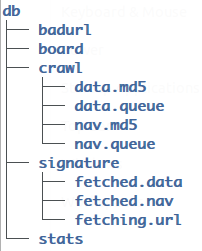
\includegraphics[]{figs/db_tree.png}

  各个目录的存放数据如下表所示:
  \begin{tabular}{| p{0.35\textwidth} | p{0.6\textwidth}|}
    \hline
    \rowcolor{red!10}
    目录名称 & 存放数据 \\ \hline
    db/badurl &  保存了所有的坏链和不存在的主机地址 \\ \hline
    db/board & 保存了所有的采集任务,每个任务代表某个频道的监控源 \\ \hline
    db/crawl/data.md5 & 在数据库中排队等待抓取的文章URL签名\\ \hline
    db/crawl/data.queue & 在数据库中排队等待抓取的文章URL队列 \\ \hline
    db/crawl/nav.md5 & 在数据库中排队等待抓取的列表URL签名\\ \hline
    db/crawl/nav.queue & 在数据库中排队等待抓取的列表URL队列\\ \hline
    db/signature/fetched.data & 已经采集过的文章URL的MD5签名 \\ \hline
    db/signature/fetched.nav & 已经采集过的列表页URL的MD5签名 \\ \hline
    db/signature/fetching.url & 分配给某个爬虫客户端正在抓取的URL的MD5签名,2分钟自动失效
    \\ \hline
    db/stats & 抓取统计数据,如每天、每小时抓取的文章数量 \\ \hline
  \end{tabular}
  
\end{center}




\end{document}

%%% Local Variables:
%%% mode: latex
%%% TeX-master: t
%%% End:
